%%%%%%%%%%%%%%%%%%%%%%%%%%%%%%%%%%%%%%%%%%%%%%%%%%%%%%%%%%%%%%%%%%% 
%                       rpithes-short.tex                         %
%         Template for a short thesis all in one file             %
%        (titlepage info below assumes masters degree}            %
%  Just run latex (or pdflatex) on this file to see how it looks  %
%      Be sure to run twice to get correct TOC and citations      %
%%%%%%%%%%%%%%%%%%%%%%%%%%%%%%%%%%%%%%%%%%%%%%%%%%%%%%%%%%%%%%%%%%% 
%
%  To produce the abstract title page followed by the abstract,
%  see the template file, "abstitle-mas.tex"
%
%%%%%%%%%%%%%%%%%%%%%%%%%%%%%%%%%%%%%%%%%%%%%%%%%%%%%%%%%%%%%%%%%%%

\documentclass{thesis}
\usepackage{graphicx}

% Use the first command below if you want captions over 1 line indented.
% A side effect of this is to remove the use of bold for captions. 
% To restore bold, also include the second line below.
%\usepackage[hang]{caption}     % to indent subsequent lines of captions
%\renewcommand{\captionfont}{\bfseries} % only needed with caption package;
                                        %   otherwise bold is default)
                                        
%%%%%%%%%%%%%%%%%%%%  supply titlepage info  %%%%%%%%%%%%%%%%%%%%%
\thesistitle{\bf Thin Shell Structure Design Tool}        
\author{R. Allan Pendergrast}
\degree{Master of Science}
\department{Computer Science}
\thadviser{Barbara M. Cutler}
\submitdate{May 2010\\(For Graduation May 2010)}        
%\copyrightyear{1685}  % if date omitted, current year is used. 
%%%%%%%%%%%%%%%%%%%%%   end titlepage info  %%%%%%%%%%%%%%%%%%%%%%
      
\begin{document} 
\titlepage             % Print titlepage   
%\copyrightpage        % optional         
\tableofcontents       % required 
\listoftables          % required if there are tables
\listoffigures         % required if there are figures

\specialhead{ACKNOWLEDGMENT}
Thanks to Barbara Cutler for all her help in creating, testing, and writing about this tool.

\specialhead{ABSTRACT}
Thin-shell structures are becoming increasingly useful in construction and design of buildings.  They allow the usage of less material to enclose
larger spaces, are structurally efficient, and have a natural aesthetic beauty.  However, they can be difficult to design, as the exact shape
required for structural stability depends on the material used, the size of the shell, and other features.  Fortunately, it is possible to simulate
these structures quickly and accurately, allowing architects to concentrate more on their design and less on ensuring that their building is
stable.  The tool described in this thesis simulates thin-shell structures and aids architects in their design and optimization.

\chapter{INTRODUCTION}

\section{Project Goals}
This project was originally conceived as a structural analysis tool that would find highly over- or underloaded members in a structure
and notify the architect that some force could be diverted towards the less-used member or that the underloaded member could be
removed.  This redesigning would help to optimize the structure, resulting in a structure that required less material or work to construct.
Since then, the focus has shifted to the design and optimization of thin shell structures.  These structures, covered in more detail in
\ref{thinshell}, are used in architecture to conserve materials, funds, or for simply aesthetic reasons.  Unfortunately, thin-shell
structures have been famously difficult to optimize and construct, sometime requiring a complete overhaul of the structure to fix stability
problems. This tool attempts to alleviate this difficulty and make the design and optimization of such structures easier and faster for architects.

\section{Terms Used}
\begin{itemize}
\item Catenarian: The shape made by a hanging chain, described by the hyperbolic cosine function.
\item Thin Shell Structure: A light weight construction which supports itself.
\end{itemize}

\section{Related Works}
\subsection{Procedural Modeling}
In "Procedural Modeling of Strucutrally-Sound Masonry Buildings", Whiting, Ochsendorf, and Durand explore
the possibilities of creating existing or novel structures procedurally.  They began by creating a grammar
which can be used to construct masonry buildings.  Arches, buttresses, domes, and vaults are some of the
structural elements which are then combined in their software.  These grammar elements are assembled into
a structure through a procedural algorithm which cuts windows in walls and assembles
all the various masonry elements of the building.  Once the initial configuration is
generated, the software runs static analysis on the building.  If it is feasibly stable, the program is
done.  If not, the program determines a measure of infeasibility, which is a measure of how far away from
stable a structure is.  The static analysis only allows for compressive forces, as the tensile strength of
masonry elements is close to zero.  Friction is also modeled, allowing for some shear.  Once the measure
of infeasibility is calculated, a parameter search is conducted iteratively, searching the parameter space
for a stable configuration.  Depending on the application, this stable configuration will take into account
a factor of safety.  The more likely a structure is to have changing loads, the higher a factor of
safety is needed.  For example, a bridge needs a higher factor of safety than a cathedral.  In the event
that there is no feasible configuration for a structure, the least infeasible structure is returned and the
user is required to add new structural elements.

In "Creating Models of Truss Structures with Optimization", Smith, Hodgins, Oppenheim, and Witkin propose
a method of creating trusses procedurally.  This work allows the user to define several anchor points
and loads for a truss, then have the software automatically generate a truss.  In this work, the risk
of pieces falling apart is not an issue as it was in the previous paper.  The primary failure method
in this case is buckling, since all forces are axial.  Therefore, the core of the algorithm is a
multivariable optimization with constraints.  The algorithm attempts iteratively to minimize weight
while ensuring that none of the members will fail, either in tension or compression.

My work had initially intended to go in this direction, using static analysis of structures within
Google Sketchup.  However, Sketchup proved to be a poor environment for the program I wanted to write, so
the project was moved to a standalone application and the focus shifted to thin-shell structures.

\chapter{THIN SHELL STRUCTURES} \label{thinshell}

\section{What are they?}
A thin shell structure is a structure which has a small thickness compared to its other dimensions.  While this may seem to be
an obvious definition, the design and construction of these structures can be complicated.  Unlike normal beam and plate structures,
thin shell structures are curved, which allows the force to travel through the thinner structural elements.  See \ref{stability} for
more information on the stability of thin shell structures.  Thin shell structures are used often in construction when a large interior
space is desired, since they do not require any interior columns if designed correctly.  Some prominent thin shell structures include
the TWA Flight Center Building at the JFK International Airport in New York, New York, the Kresge Auditorium on the MIT campus in
Cambridge, Massachusetts, and the Montreal Biosphere in Montreal, Canada.

\section{Why do we care?}
Since the force travels directly through the structural elements in a thin shell structure, these structural elements can be thin.  This
thinness results in less material being used, which can save money for the companies involved.  Furthermore, since the structure supports
itself, it offers a large uninterrupted interior space, which can be used for any number of applications.


\chapter{THIN SHELL OPTIMIZATION}

\section{Building Stability} \label{stability}
In order for a building to stand up, the lines of thrust must pass through structural elements.  As can be seen in Figure \ref{FIGURE_arch_lines},
traditional arches must be rather thick to contain the lines of thrust produced by their weight.  However, a catenarian arch can be built
much thinner for the same stability, as it contains the line of thrust exactly.
To extrapolate to entire buildings, traditional construction methods require very thick elements to be used in order to keep the lines of thrust
within a building's structural elements.  However, if the shape of the building is instead matched to the shape of the lines of thrust, the
structural elements can be much thinner, needing only to support the direct compressive force.
\begin{figure}
\resizebox{4in}{!}{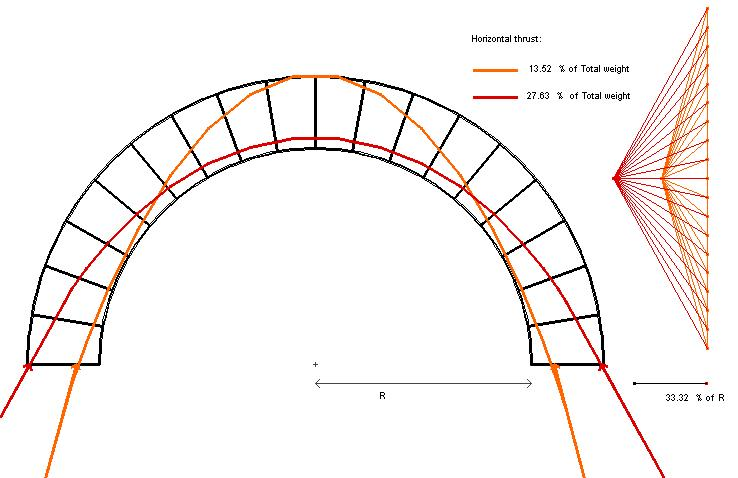
\includegraphics{images/arch.png}}
\caption{Lines of thrust}
\label{FIGURE_arch_lines}
\end{figure}

\section{Hanging Chains}
Hanging chains have been used by architects, most famously Antoni Gaud\'{i}, to design structures for stability and aesthetics.  Since a hanging
chain is supporting itself purely in tension and a catenary arch is supporting itself purely in compression, one can be used to describe the other.
More complicated systems of hanging chains and weights can and have been used to design a number of structures, including the Sagrada Familia in
Barcelona, Spain.  Design by hanging chains offers a relatively quick and accurate turnaround time, but it is still tedious to adjust the chains
to find the desired shape.  Furthermore, inverting the model can be a tedious and confusing process.  Fortunately, hanging chains are simple to simulate.

\section{Cloth}
A standard cloth simulation shares many similarities with the hanging chains model.  A finite number of elements connected by links will, when
submitted to gravity, form a catenary.  In cloth simulation, a finite number of points exert forces on each other, falling into a tensionally stable
configuration.  Additionally, since the model is simulated, gravity can be reversed and the model shown as it would be built, making it easier for
the architect to visualize the completed structure.

\chapter{THIN SHELL DESIGN TOOL}

\section{Layout}
As can be seen in figure \ref{FIGURE_screenshot}, there are 3 main panels in the design tool.  On the left is the viewing panel, where the structure
is shown in 3D.  This view can be rotated, zoomed, and panned to give the architect the view they need.  There is no actual interaction with the
structure in this panel; all of the interaction is done via the two right-hand panels.  The top-right panel is the floorplan panel.  This panel
contains a point for each point of the structure that is in contact with the ground.  These points can be moved around in order to modify the shape
of the structure to fit the architect's vision.  The bottom-right panel is the grid panel.  This panel shows all the vertexes of the structure in 2D.
This panel can be used to disable points, creating voids in the structure.  It can also be used to associate different points in the shell with certain
points in the floor plan.  This is most useful when adding new points to the floor plan, allowing the architect to define a new point of support on the
fly.  Together, these windows allow the architect broad control over the design of their structure, while the tool works in the background to keep the
shape of the structure optimal.
\begin{figure}
\resizebox{5in}{!}{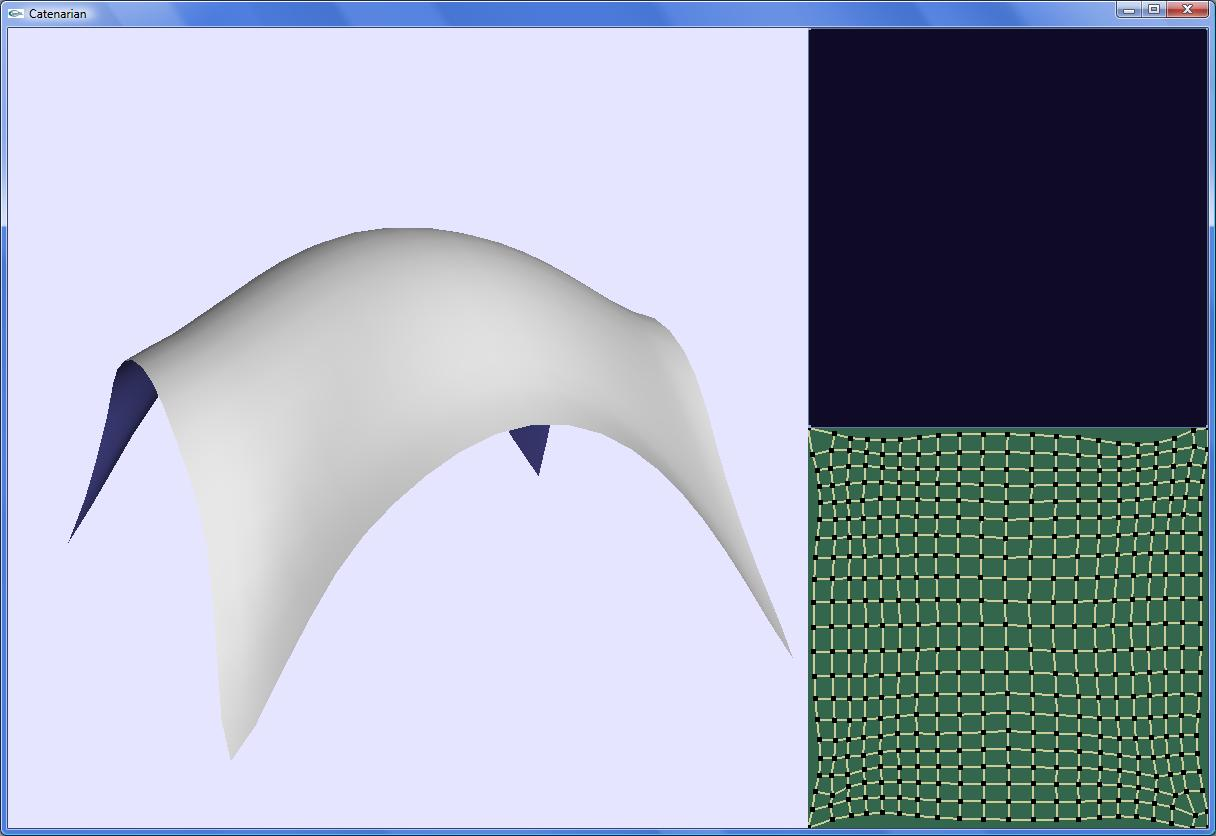
\includegraphics{images/screenshot.png}}
\caption{A screenshot of the tool}
\label{FIGURE_screenshot}
\end{figure}

\section{Simulator}
The heart of the tool is the simulator.  This simulator uses a second-order explicit integral solver to simulate the forces on the structure.  These forces
cause the structure to form catenaries, shapes that will support themselves.  The floorplan, grid, and viewing window can all be interacted with in real
time while the simulation is going on, allowing the architect to make changes on the fly.  Depending on the magnitude of the changes made, the simulator
will take anywhere from a second to a couple minutes to reach equilibrium.  It should be noted that until the simulation does reach equilibrium there are
no guarantees of the stability of the structure.


% The following produces a numbered bibliography where the numbers
% correspond to the \cite commands in the text.
\specialhead{LITERATURE CITED}
\begin{singlespace}
\begin{thebibliography}{99}
\bibitem{thisbook} There are no books cited yet.
\end{thebibliography}
\end{singlespace}

%%%%%%%%%%%%%%%%%%%%%%%  For Appendices  %%%%%%%%%%%%%%%%%%%
%\appendix    % This command is used only once!
%\addtocontents{toc}{\parindent0pt\vskip12pt APPENDICES} %toc entry, no page #
%\chapter{THIS IS AN APPENDIX}
%Note the numbering of the chapter heading is changed.
%This is a sentence to take up space and look like text.
%\section{A Section Heading}
%This is how equations are numbered in an appendix:
%\begin{equation}
%x^2 + y^2 = z^2
%\end{equation} 
%
%\chapter{THIS IS ANOTHER APPENDIX}
%This is a sentence to take up space and look like text.
%
\end{document}
